\chapter{Measurements}
\label{kap-measure}

\section{Introduction}

\section{Study Area and Instrumentation}

We obtained hydrographic and turbulence data at 
several locations throughout the German coastal area during three cruises with 
R/V \textit{Alkor} in spring 2014 (AL434, 28.03.-08.04.2014), R/V 
\textit{Elisabeth Mann Borgese} in spring 2015 (EMB100, 09.04.-16.04.2015) and 
R/V \textit{Maria S. Merian} in winter 2016 (MSM50, 05.01.-29.01.2016). Here, 
we exclusively discuss data obtained in the transition zone from the coast off 
the island R\"{u}gen (called Tromper Wiek (TW), around 30~m water depth) to 
the approximately 45~m deep Arkona Basin (AB). The exact positions of deployed 
moorings and ship-based microstructure profiler transects are indicated in 
\fig{studyarea}.
 \begin{figure}[ht]
 \centering
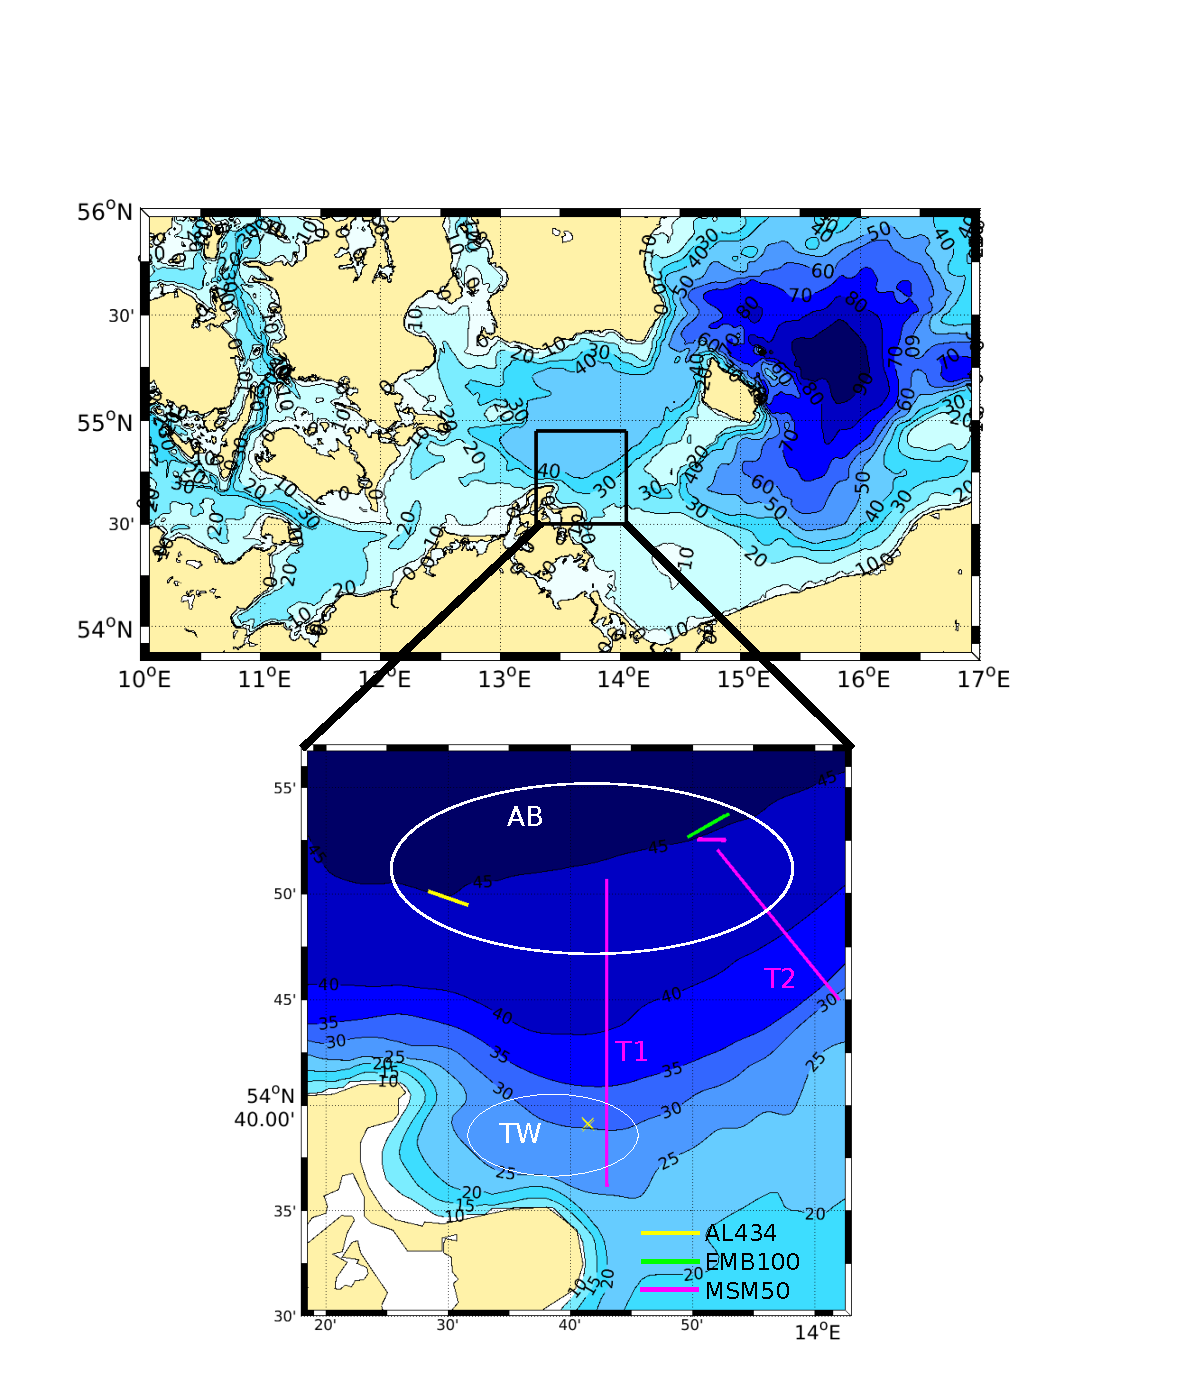
\includegraphics[width=17cm]{bilder/studyarea.pdf}
 \caption{(A) Western Baltic Sea and (B) enlargement of the study area. 
Deployments during cruise AL434 are indicated in yellow, from EMB100 in green 
and from cruise MSM50 in magenta.}
 \label{studyarea}
 \end{figure}

Sediment distribution in this area is heterogeneous in the shallow regions with 
predominately medium to fine sand. At water depths below 25 - 30~m in the 
Arkona Basin, sediment is finer and consists homogeneously of silt 
(\fig{tauberkarte}). In the vicinity of TW, a special type of fine grained and 
organic poor sediment is found. Previous studies \citep[][]{leipe2000, 
basys1} found the Arkona Basin to be a deposition center for material 
orginiating from the shallower areas, with accumulation rates of around 2.2 
mm/yr. Sediment characteristics in the Arkona Basin resemble to those of a 
fluffy layer, i.e. it is easily resuspended and, due to its low settling 
velocity, remains suspended for a relatively long period of time. A consecutive 
study \citep[][]{basys2} found the 20~m isobath to be the border between 
erosional and depositional sites in this area, yielding that the Tromper Wiek 
region is depositional as well. This study also pointed out that muddy 
sediments accumulated below the halocline in this region.
 \begin{figure}[ht]
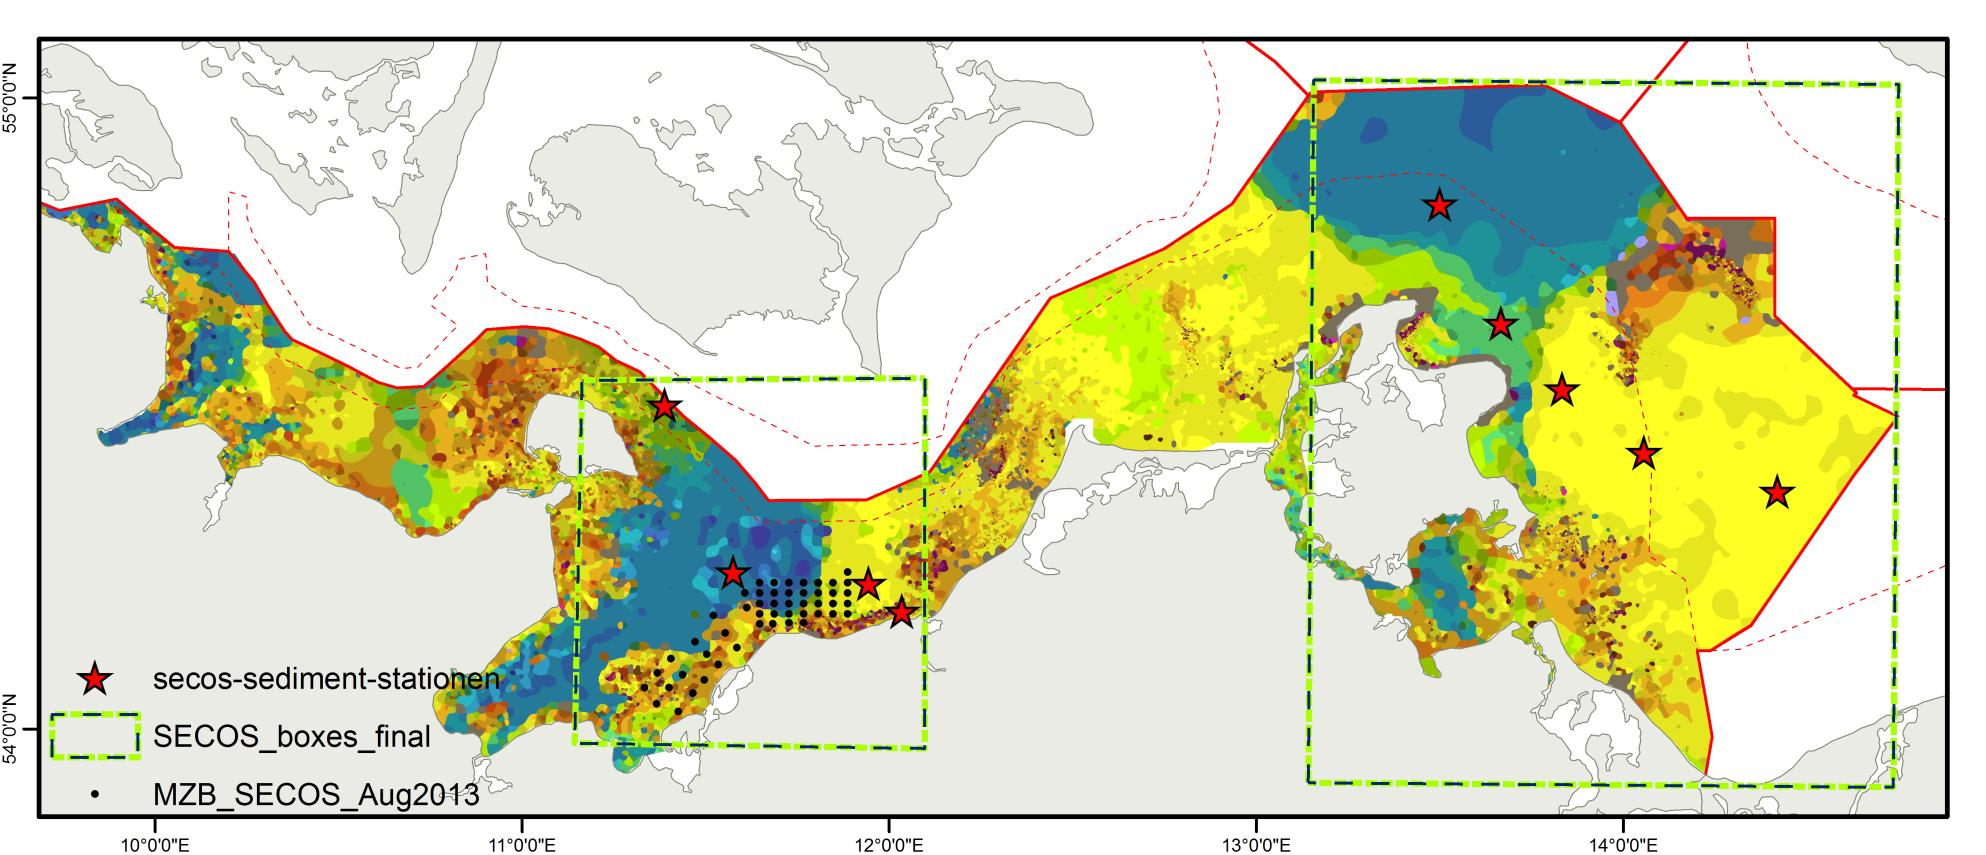
\includegraphics[width=20pc]{bilder/bild.png}
 \caption{Sediment distribution in the Western Baltic Sea. Besser Karte mit 
Legende. Tauber und BSH.}
 \label{tauberkarte}
 \end{figure}

Three different types of moorings were deployed: A CTD-Chain consisted of eight 
CTD-loggers (MicroCat from Seabird, USA), tied to a mooring line at intervals 
of 1 m, starting at 1 m above the seabed, additionally two optical 
backscatter sensors (NTU from Wetlabs, USA) at 3.5 and 5.5 m above the seabed. 
For the EMB100 cruise, the CTD-Chain was extended to 10 CTD-loggers (5 MicroCat 
and 5 TR-1060 type from RBR, Canada) and the turbidity sensors were omitted. 
Lander 1 was a bottom-mounted instrument frame with an upward looking 1200 kHz 
ADCP (Teledyne RDI, USA), a 6 MHz single-point Doppler current meter (Vector 
from Nortek AS, Norway), another CTD-logger and a turbidity sensor. Lander 2 
was a similar bottom frame equipped with an upward looking 600 MHz ADCP 
(Teledyne RDI, USA) and an upward looking 1 MHz (2 MHz during cruise AL434) 
pulse-coherent ADCP (Aquadopp HR from Nortek AS, Norway). For the cruises 
EMB100 and MSM50, Lander 2 was complemented with an additional CTD-logger and a 
turbidity sensor. Deployment times of the moorings are listed in 
\tab{deployments}.

Ship-based microstructure measurements were performed with a MSS90-L 
microstructure profiler (ISW, Germany). The instrument contained a set of 
precision CTD sensors, a fast FP07 thermistor, a turbidity sensor, and two 
airfoil shear-probes. During the transects (each of 1 to 5 hours duration) the 
ship moved at 1-2 kn and profiles were obtained continously. Number and time of 
the transects for each cruise are summarized in \tab{mss}.

 \begin{table}
\caption{Deployment times of moorings (UTC). In the first 
line, TW and AB indicate deployment sites near the coast and in the Arkona 
Basin, respectively.}\label{deployments}
\begin{center}
\begin{tabular}{cccc}
\hline
\hline
 & AL434 (TW) & EMB100 (AB) & MSM50 (TW) \\
 \hline
 start & 03.04.2014, 07:00 & 14.04.2015, 12:00 & 26.01.2016, 22:00 \\ 
 end & 08.04.2014, 06:00 & 17.04.2015 04:00 & 28.01.2016, 07:00 \\
\hline
 & CTD-Chain & CTD-Chain & \\
 & Lander 1 & Lander 1 & Lander 1\\
 & Lander 2 & Lander 2 & Lander 2\\
\hline
\end{tabular}
\end{center}
\end{table}

 \begin{table}
\caption{Start and end times (UTC) and number (in brackets) of microstructure 
transects.}\label{mss}
\begin{center}
\begin{tabular}{cccc}
\hline
\hline
 & AL434 (2014) & EMB100 (2015) & MSM50 (2016)\\
 \hline
Tromper & 04.04., 16:15 - & & 27.01., 00:00 - \\ 
Wiek & 04.04., 22:30 (4) & & 28.01., 06:00 (9)\\
 & 06.04., 17:30 & & \\
 &  07.04., 22:15 (8) & & \\
\hline
Arkona & 05.04., 16:15 - & 14.04., 16:45 - & 23.01., 13:30 - \\
Basin & 06.04., 01:15 (5) & 15.04., 05:30 (5) & 24.01., 16:45 (7)\\
\hline
transect &  & & 24.01., 19:30 - 23:45 (T1)\\
coast to basin & & & 28.01., 09:45 - 17:00 (T2)\\
\hline
\end{tabular}
\end{center}
\end{table}

\section{Observations}

\subsection{Tromper Wiek}

During the 5 day instrument deployment in 2014 (\tab{deployments}), we captured 
a storm event with 7 Bft wind and up to 4 m wave height with a consecutive calm 
period (\fig{tromperwiek}, a). In \fig{tromperwiek}, b the variance of the 
horizontal velocity componentsfiltered for wave periods between 2 and 20 
seconds, which is proportional to the kinetic energy contained in the 
waves, is displayed. Although wave energy was maximal in the afternoon of April 
4, the peak in turbidity was not reached until late morning of April, 5. This 
yields that local resuspension during storm did not occur, but a turbid 
watermass was advected to the measurement site. Near bottom current 
(\fig{tromperwiek},C) was directed to the south during the relevant period, i.e. 
water from deeper parts was advected up the slope.
 \begin{figure}[ht]
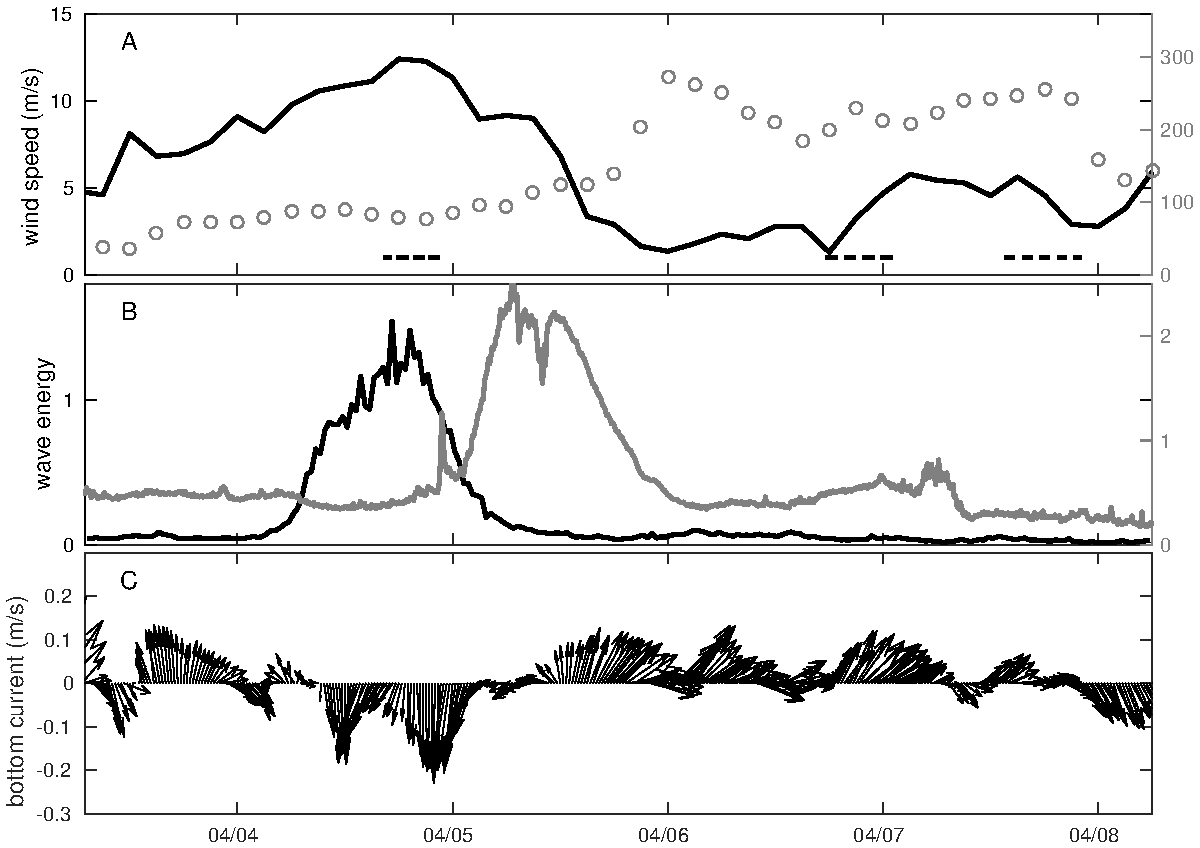
\includegraphics[width=15cm]{bilder/al434tw.pdf}
 \caption{(A) Wind speed and direction from the hindcast of the German Weather 
Service, (B) wave energy and turbidity and (C) direction of 
near bottom current, all obtained with Lander 1 during the deployment at TW on 
cruise 
AL434.}
 \label{tromperwiek}
 \end{figure}

In the CTD Chain data in \fig{ctdchain} we see a steady increase of the 
near-bottom salinity, accompanied by increasing turbidity. The increase in 
turbidity is clearly linked to the increase of salinity, supporting that turbid 
water is advected to TW from deeper regions below the halocline.

 \begin{figure}[ht]
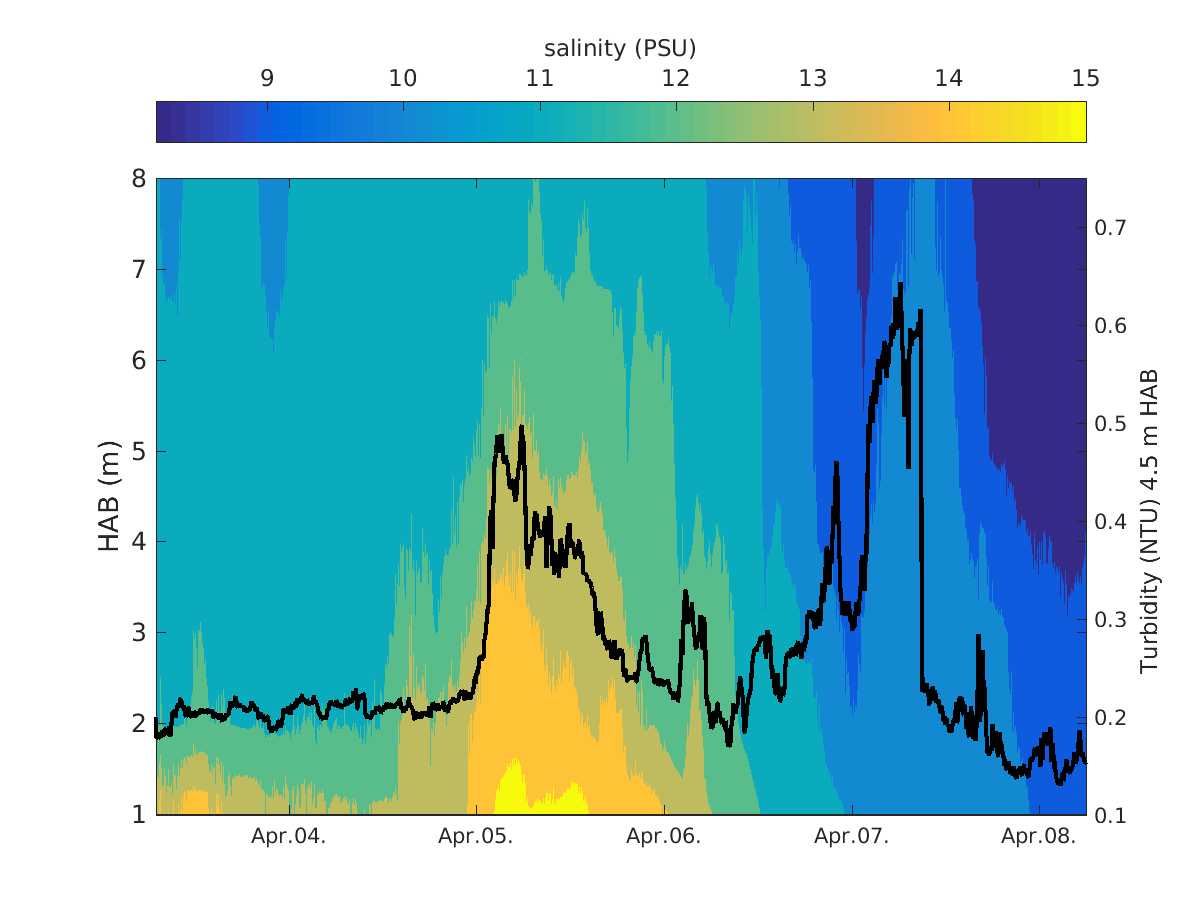
\includegraphics[width=15cm]{bilder/ctdchaintw.png}
 \caption{Salinity (PSU) obtained from the CTD Chain deployed at Tromper Wiek 
during cruise AL434.}
 \label{ctdchain}
 \end{figure}

 This advection of saline water near the bottom is triggered by the local wind 
forcing. Strong easterly wind causes Ekman transport to the north in the 
surface layer \citep[][]{lass2001}, which is visible in the velocity data from 
the 600~kHz ADCP mounted on Lander~2. After the wind decayed, 

\subsection{Transect}

In \fig{transect} we see how the water body is structured along the slope from 
the coast into the basin. A sharp halocline seperates a turbulent bottom 
boundary layer (BBL) of approximately 5 m from the interior. At the left hand 
side of the pannel, where the slope angle steepens, the halocline is widened. 
The boundary layer is generally turbid: Turbidity is more patchy at the upper 
parts of the slope, but high values are confined to the bottom boundary layer, 
so no suspended matter is mixed across the halocline. This indicates that 
turbidity is caused by material originating from the seafloor and held in 
suspension by turbulent motions in the BBL.
Salinity isolines are rather parallel to the slope than straight horizontal, 
what would be the stably stratified case.
  \begin{figure}[ht]
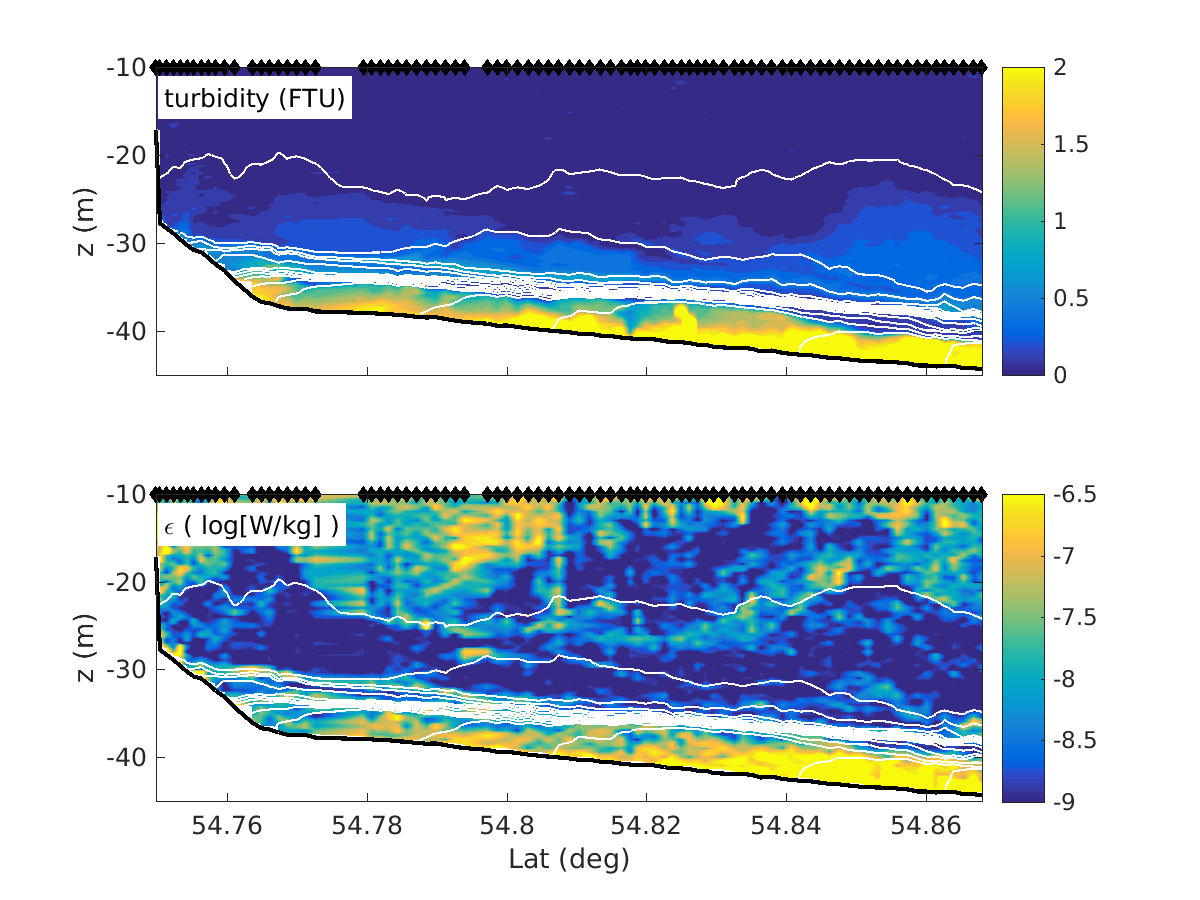
\includegraphics[width=15cm]{bilder/abtrans.png}
 \caption{Turbidity and dissipation rate from the microstructure transect T2. 
White lines indicate levels of equal salinity.}
 \label{transect}
 \end{figure}


\subsection{Arkona Basin}

During each of the three cruises, we collected microstructure data in the 
Arkona Basin. \fig{abmss} shows the profiles of dissipation rate and turbidity, 
averaged over all profiles obtained in the basin for each cruise. A turbulent 
BBL is visible in all three profiles, ranging from 1 to 5 m thickness. 
Turbidity is again enhanced in the BBL, but not above, supporting the data 
described in the last section. As this data set was obtained over three years 
and in different seasons, it is most likely that this turbid, very sharply 
defined BBL is constantly present in the Arkona Basin.
   \begin{figure}[ht]
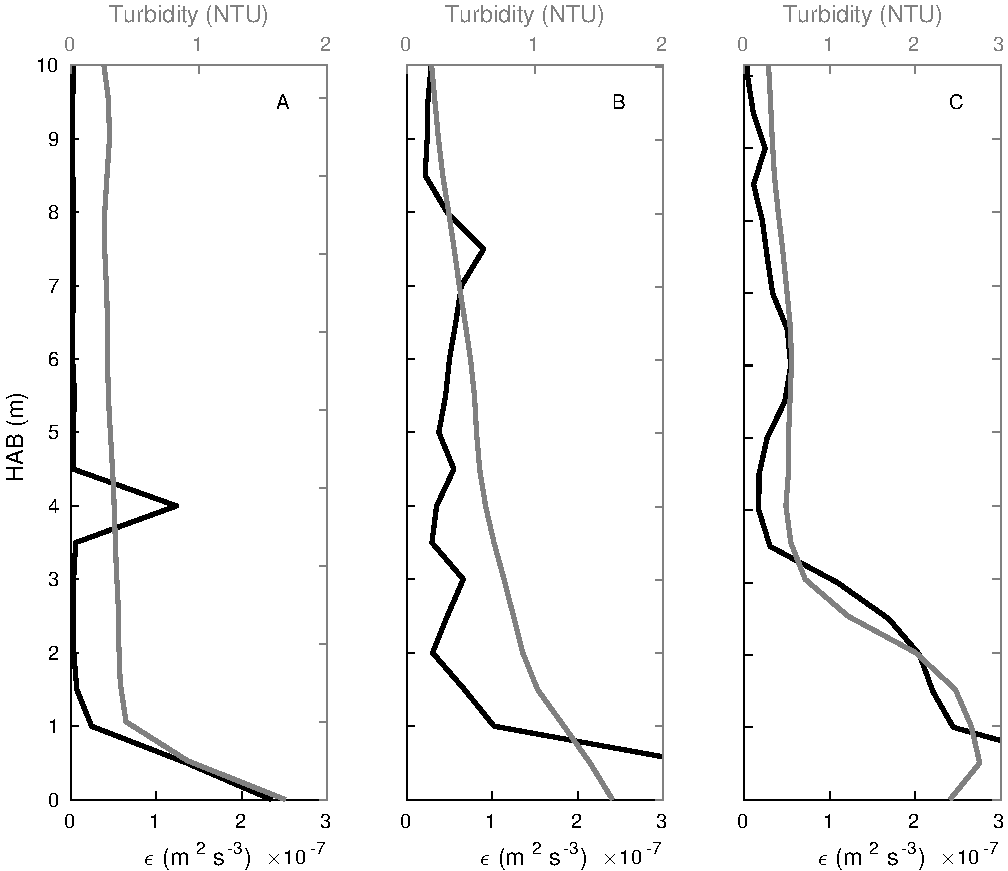
\includegraphics[width=15cm]{bilder/arkona_mss.pdf}
 \caption{Turbidity and dissipation rate from all microstructure transect in 
the Arkona Basin. Solid lines are mean values, dashed line the standard 
deviation. Only the lowermost part of the watercolumn is displayed here.}
 \label{abmss}
 \end{figure}
 
\section{Discussion}

\section{Conclusions}